% !TeX program = pdflatex
\documentclass[11pt,a4paper]{article}
\usepackage{kotex}
\usepackage{geometry}
\geometry{top=3cm,bottom=3cm,left=2.5cm,right=2.5cm}
\usepackage{graphicx,amsmath,amssymb,mathtools,bm,booktabs,float,array}
\usepackage{caption,indentfirst,enumitem,xurl,hyperref}
\usepackage[strings,nohyphen]{underscore}
\captionsetup[figure]{font=small,labelfont=bf,skip=8pt}
\captionsetup[table]{font=small,labelfont=bf,skip=8pt}
\hypersetup{colorlinks=true,linkcolor=blue,filecolor=magenta,urlcolor=cyan,
 pdftitle={전자기파와 광학 연습},pdfauthor={이동규 2021-11538}}
\renewcommand{\thesection}{문제 \arabic{section}.}
\renewcommand{\thesubsection}{\arabic{section}.\arabic{subsection}}
\renewcommand{\thesubsubsection}{\arabic{section}.\arabic{subsection}.\arabic{subsubsection}}
\pagestyle{plain}
\setlength{\parindent}{1em}
\setlength{\parskip}{0.4em}
\linespread{1.15}
\setlist{leftmargin=1.5em,topsep=0.4em,itemsep=0.2em,parsep=0.1em}
\widowpenalty=10000\clubpenalty=10000\displaywidowpenalty=10000
\raggedbottom
\setlength{\emergencystretch}{3em}
\newcommand{\dd}{\mathrm{d}}\newcommand{\ee}{\mathrm{e}}
\newcommand{\unit}[1]{\,\mathrm{#1}}
\newcommand{\sci}[2]{\mathord{#1\times10^{#2}}}
\newcommand{\pairplot}[2]{\par\addvspace{0.4em}\noindent
\begin{minipage}{\linewidth}\centering
\includegraphics[width=0.96\linewidth]{images/#1.pdf}
\captionof*{figure}{#2}\end{minipage}\par\addvspace{0.5em}}
\title{\huge\textbf{전자기파와 광학 연습}\\[0.5em]
 \large Propagation of an Electromagnetic Wavepacket}
\author{이동규 2021-11538}
\date{}
\begin{document}
\maketitle
\section{토의 및 AI 사용 공개}
\noindent\textbf{함께 토의한 사람:} 함께 토의한 사람 없음\par
\noindent\textbf{사용한 AI (이름 및 버전):} GPT-6.1 Sol\par
\noindent\textbf{입력한 질문}\par
\begin{enumerate}[label=\arabic*.,leftmargin=1.8em,itemsep=0.35em,topsep=0.4em]
\item Yee-type staggered grid에 대한 정보가 필요해, 관련 정보를 얻을 수 있는 교재나 사이트를 제안해줘. 그리고 이게 뭔지 간략히 설명하고, 이를 어떻게 구현하는지 제시해줘.
\item Leapfrog 방법이 정확히 어떻게 구현되고 왜 이 방법을 사용하는지 알려줘. 
\item 시공간을 반 칸씩 어긋나게 놓는 시간 적분 방식이 Leapfrog 방법이라는 건 알겠는데, 이게 어떤 장점이 있는지 구체적으로 설명해줘.
\item 시간 간격과 공간 간격이 구체적으로 어떤 조건에서 안정적이라고 할 수 있는거지?
\item 그래서 Yee 격자에서 전기장과 자기장의 위치와 시각을 반 칸씩 어긋나게 두는 이유가 뭐야?
\item 문제 3에서 파묶음이 $+z$ 방향으로만 진행하도록 정한 초기 자기장은 왜 그렇게 추정할 수 있나?
\item 전기장 진폭과 자기장 진폭으로 각각 반사율·투과율을 계산하는 식을 함께 제시해줘.
\item 가능한 오차 원인을 나열하는 데 그치지 않고, 실제 원인을 분리해 검증할 실험 계획을 세워줘. 그 실험을 실행하여 주된 오차 원인이 무엇인지 분석하고 검증 결과를 설명해줘.
\item simulate()에서 자기장을 먼저 계산하고 전기장을 나중에 계산하는 이유가 뭐야? 이 순서로 해야 하는 이유를 설명해줘.
\item 반복문에서 사용하는 전기장과 자기장은 각각 어느 시각의 값인 거야? 갱신 전후로 구분해서 설명해줘.
\item np.diff(e)랑 np.diff(b_plus)가 각각 어떤 미분을 계산하는 거야? 갱신식에 마이너스가 붙는 이유도 같이 설명해줘.
\item 전기장 배열이 자기장 배열보다 하나 더 긴데, 왜 이렇게 되는 거야?
\item 자기장을 그냥 \(B_y\)로 계산하지 않고 \(b=cB_y\)로 바꿔서 계산하는 이유가 있어? 그래프에서는 다시 어떻게 바꾸는 거야?
\item b_minus = b_zero + 0.5 * COURANT * np.diff(e)는 어떻게 나온 식이야? 초기 자기장을 그대로 넣으면 안 되는 건가?
\item 그래프를 그릴 때 자기장은 왜 b_minus랑 b_plus를 평균해서 사용하는 거야?
\item material_fraction이 경계에서 유전체가 차지하는 비율을 어떻게 계산하는 건지 설명해줘.
\item 출력 시각을 반복 횟수로 바꾸면서 반올림했는데, 왜 그다음에 시간 격자와 일치하는지 다시 확인하는 거야?
\item 진폭을 구할 때 그냥 배열의 최댓값을 사용하면 안 돼? 세 점으로 보간하는 이유가 뭐야?
\item 입사파, 반사파, 투과파의 진폭은 각각 어느 구간에서 구하는 거야? 반사 전기장은 음수인데 이 부호는 어떻게 처리하고 있어?
\item 그래프 코드만 수정했을 때 계산 결과는 그대로라는 걸 어떻게 확인할 수 있어? 실제로 비교해서 확인하는 방법을 설명해줘. 
\end{enumerate}
\newpage
\section{초기 자기장이 0인 진공 파묶음}
전기장 $\bm E=E_x(z,t)\hat{\bm x}$, 자기장 $\bm B=B_y(z,t)\hat{\bm y}$에 대해
Maxwell의 두 회전 방정식을 직접 시간 적분하였다. 초기장은
$E_x(z,0)=\ee^{-z^2/\sigma^2}\unit{V/m}$, $\sigma=\sci{1.00}{0}\unit m$이다.
매질은 $\mu_r=\sci{1.00}{0}$인 선형·무손실·비분산 유전체로 가정한다.
물리량과 계산 결과는 과학적 표기법으로 소수점 셋째 자리에서 반올림하였다.

\vspace{1em}
\subsection{Maxwell 방정식과 Yee 격자}
\subsubsection{방정식 정리}
자유 전하와 자유 전류가 없고, $\bm D=\epsilon(z)\bm E$,
$\bm H=\bm B/\mu_0$라고 두면 [Griffiths, §7.3.5, 식 (7.65), (7.67)]
\begin{align}
 \nabla\cdot\bm D&=0,&\nabla\cdot\bm B&=0,\\
 \nabla\times\bm E&=-\frac{\partial\bm B}{\partial t},&
 \nabla\times\bm H&=\frac{\partial\bm D}{\partial t}.
\end{align}
$E_x,B_y$는 $z,t$에만 의존하므로 두 발산식은 자동으로 만족한다.
$\nabla\cdot\bm D=\partial_x(\epsilon(z)E_x)=0$이며,
경계면에 수직인 $D_z,B_z$도 0이다. 두 회전식의 남는 성분은
\begin{equation}
 \boxed{\frac{\partial B_y}{\partial t}=-\frac{\partial E_x}{\partial z},\qquad
 \frac{\partial E_x}{\partial t}=-\frac{1}{\mu_0\epsilon(z)}\frac{\partial B_y}{\partial z}.}
 \label{eq:maxwell1d}
\end{equation}
이 식을 직접 계산한다. $\tau=ct$와 $b=cB_y$를 도입하면
\begin{equation}
 \frac{\partial b}{\partial\tau}=-\frac{\partial E_x}{\partial z},\qquad
 \epsilon_r(z)\frac{\partial E_x}{\partial\tau}=-\frac{\partial b}{\partial z}.
 \label{eq:normalized}
\end{equation}
$\tau$는 길이 단위이고 $b$는 $E_x$와 같은 단위이다.

\newpage\subsection{Yee 격자와 시간 적분}
\subsubsection{Leapfrog 방법}
$E_j^n=E_x(z_j,n\Delta t)$와
$b_{j+1/2}^{n+1/2}=b(z_j+\Delta z/2,(n+1/2)\Delta t)$를 둔다.
서로 이웃한 두 장의 차이가 해당 장 위치에서의 중심차분을 이루며,
두 장을 번갈아 갱신하는 leapfrog 방법이 된다 [Schneider, §§3.2--3.3].
\begin{align}
 b_{j+1/2}^{n+1/2}&=b_{j+1/2}^{n-1/2}-S(E_{j+1}^{n}-E_j^{n}),\\
 E_j^{n+1}&=E_j^{n}-\frac{S}{\bar\epsilon_{r,j}}
 (b_{j+1/2}^{n+1/2}-b_{j-1/2}^{n+1/2}),\qquad S=\frac{c\Delta t}{\Delta z}.
 \label{eq:yee}
\end{align}
\begin{center}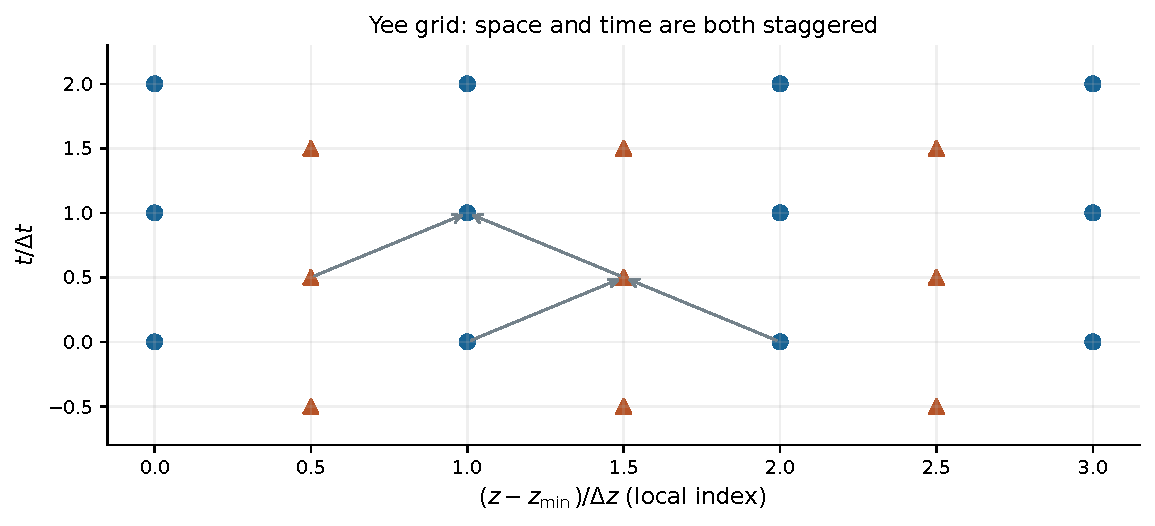
\includegraphics[width=0.91\linewidth]{images/yee_grid.pdf}\\[-0.3em]
\small \textbf{그림 1.} 전기장(원)과 자기장(삼각형)의 시공간 배치.\end{center}

\newpage
\subsection{초기 조건}
\subsubsection{초기 자기장의 시간 격자 배치}
코드는 첫 갱신 직전에 $b^{-1/2}$를 저장한다. 주어진 $b^0$를 이 배열에
그대로 넣으면 반 시간 간격의 오차가 생기므로 Faraday 법칙으로 초기화한다.
\begin{equation}
 b_{j+1/2}^{-1/2}=b(z_{j+1/2},0)+\frac{S}{2}(E_{j+1}^{0}-E_j^{0}).
 \label{eq:init}
\end{equation}
이후 첫 Faraday 갱신을 하면 $b^{+1/2}=b^0-(S/2)\Delta E^0$가 된다.
따라서 $(b^{-1/2}+b^{+1/2})/2=b^0$로서 지정한 초기장이 재현된다.

모든 자기장 그래프에는
\begin{equation}
 B_y(z_{j+1/2},t_n)\simeq
 \frac{b_{j+1/2}^{n-1/2}+b_{j+1/2}^{n+1/2}}{2c}
 \label{eq:sync}
\end{equation}
를 사용한다. 전기장과 자기장의 표시 시각은 같다. 공간 좌표는 각각
$z_j,z_{j+1/2}$를 그대로 사용하므로 공간 보간이 필요 없다.
사용된 값은 다음과 같다.
\begin{center}\small\renewcommand{\arraystretch}{1.22}
\begin{tabular}{ll}\toprule
항목 & 사용값\\\midrule
$c$ & $\sci{3.00}{8}\unit{m/s}$\\
$\mu_0$ & $\sci{1.26}{-6}\unit{H/m}$\\
$\epsilon_0$ & $\sci{8.85}{-12}\unit{F/m}$\\
계산 영역 & $\sci{-2.00}{1}\le z\le\sci{2.00}{1}\unit m$\\
$\Delta z$, $S$ & $\sci{1.00}{-2}\unit m$, $\sci{5.00}{-1}$\\
$\Delta t$ & $\sci{1.67}{-11}\unit s$\\
격자 수 & $E$: $\sci{4.00}{3}$개, $B$: $\sci{4.00}{3}$개\\
4번 매질 & $z<\sci{5.00}{0}\unit m$: $\epsilon_r=\sci{1.00}{0}$; $z>\sci{5.00}{0}\unit m$: $\epsilon_r=\sci{4.00}{0}$\\
시간 간격 조건 & $v\Delta t/\Delta z\le1$; 진공 $\sci{5.00}{-1}$, 매질 $\sci{2.50}{-1}$\\\bottomrule
\end{tabular}\end{center}

\subsubsection{매질 경계와 경계 조건}
$E_j$에 대응하는 dual cell은 $[z_j-\Delta z/2,z_j+\Delta z/2]$이다.
Ampère 법칙을 이 cell에 적분하여
\begin{equation}
 \bar\epsilon_{r,j}=\frac{1}{\Delta z}
 \int_{z_j-\Delta z/2}^{z_j+\Delta z/2}\epsilon_r(z)\,\dd z
\end{equation}
를 사용한다. 경계 $z=\sci{5.00}{0}\unit m$의 격자점에 대응하는 셀은
진공과 유전체를 절반씩 포함한다. 따라서 이 격자점의 유효 상대 유전율은
두 영역의 상대 유전율을 평균한 $\bar\epsilon_r=(1+4)/2=\sci{2.50}{0}$이다.

양 끝에는 $E=0$을 두었다. 관찰 시간은 $ct\le\sci{1.00}{1}\unit m$이고, 가장 왼쪽
중심은 $z=\sci{-1.00}{1}\unit m$에만 도달한다. 끝에 도달하는 Gaussian 꼬리의
최대 크기는 대략 $\tfrac12\ee^{-100}\unit{V/m}$이므로 주요 결과에
계산 영역 끝의 반사는 영향을 주지 않는다.

\newpage
\subsection{진공 파묶음의 시간 변화와 계산 결과}
$g(z)=E_0\ee^{-z^2/\sigma^2}$라 두자. 식 (\ref{eq:normalized})의 진공식에서
$w_+=E_x+b$, $w_-=E_x-b$를 정의하면
\begin{equation}
 (\partial_\tau+\partial_z)w_+=0,\qquad(\partial_\tau-\partial_z)w_-=0.
 \label{eq:characteristics}
\end{equation}
즉 $w_+$는 오른쪽으로, $w_-$는 왼쪽으로 이동한다.
$b(z,0)=0$이면 $w_+(z,0)=w_-(z,0)=g(z)$이므로
\begin{align}
 E_x(z,t)&=\tfrac12[g(z-ct)+g(z+ct)],\\
 B_y(z,t)&=\frac{1}{2c}[g(z-ct)-g(z+ct)].\label{eq:q2ref}
\end{align}
앞서 정리한 Maxwell 방정식을 더하고 빼면 위의 식을 얻는다. 따라서 초기 $B=0$이어도
$\partial_t B_y=-\partial_z g$는 일반적으로 0이 아니므로 장이 변한다.

두 중심이 $\sci{2.00}{0}\unit m$ 이동하는 시각은
\begin{equation}t_2=\frac{\sci{2.00}{0}\unit m}{c}=\sci{6.67}{-9}\unit{s}.\end{equation}
중심은 $z=\pm\sci{2.00}{0}\unit m$이고, 각 전기장 진폭은 약 $\sci{5.00}{-1}\unit{V/m}$이다.

자기장 진폭은 왼쪽 $\sci{-1.67}{-9}\unit{T}$, 오른쪽 $\sci{+1.67}{-9}\unit{T}$이다.
\pairplot{q2_fields}{\textbf{그림 2.} $t=2/c$의 $E_x(z)$와 $B_y(z)$.}


\newpage
\section{$+z$ 방향으로만 진행시키는 초기장}
진공에서 $+z$ 방향으로 진행하는 파는 $cB_y=E_x$, $-z$ 방향으로
진행하는 파는 $cB_y=-E_x$를 만족한다. 따라서 주어진 장을 두 진행 성분으로
분해하면 전기장은 각각 $E_{+z}=(E_x+cB_y)/2$,
$E_{-z}=(E_x-cB_y)/2$이다. $+z$ 방향으로만 진행시키려면 처음부터
$E_{-z}(z,0)=0$이 되도록 $B_y(z,0)=E_x(z,0)/c$로 정하면 된다.
식 (\ref{eq:characteristics})에 의해 이렇게 제거한 $-z$ 방향 진행 성분은 이후에도
0으로 유지된다. 문제 2와 같은 초기 전기장을 대입하면 필요한 초기 자기장은
\begin{equation}
 \boxed{\bm B(z,0)=\frac{E_0}{c}\ee^{-z^2/\sigma^2}\hat{\bm y}
 =3.34\times10^{-9}\ee^{-z^2/\sigma^2}\hat{\bm y}\unit T.}
 \label{eq:q3init}
\end{equation}
즉, 전기장과 같은 Gaussian 형태의 자기장을 $+y$ 방향으로 주고,
진폭을 전기장의 $1/c$배로 정한 것이다. 이때 $\bm E\times\bm B$는
$+\hat{\bm z}$를 향하며, 교재의 $\bm B=(1/c)\hat{\bm k}\times\bm E$와도
일치한다 [Griffiths, §9.2.2, 식 (9.47)--(9.50)].

이 초기조건으로 Yee 계산을 다시 수행하였다. 한편 해당 진행파의 식은
\begin{equation}E_x(z,t)=g(z-ct),\qquad B_y(z,t)=g(z-ct)/c.\label{eq:q3ref}\end{equation}
$t=2/c=\sci{6.67}{-9}\unit{s}$에서 중심은 $z=\sci{2.00}{0}\unit m$이다.

전기장 진폭은 $\sci{1.00}{0}\unit{V/m}$, 자기장 진폭은 약 $\sci{3.34}{-9}\unit{T}$이다.
\pairplot{q3_fields}{\textbf{그림 3.} 문제 3의 $t=2/c$ 결과.}


\newpage
\section{$z=\sci{5.00}{0}\unit m$에서의 반사와 투과}
\subsection{관찰 시각과 예상되는 위치}
문제 2의 초기장 $B_y(z,0)=0$으로 돌아간다.
오른쪽으로 가는 중심은 $5/c$에 경계에 도달하고, 반사 후 다시 $5/c$를
이동하여 원점으로 돌아온다. 따라서 마지막 시각과 10등분 시각은
\begin{equation}
 t_{\rm return}=\frac{\sci{1.00}{1}\unit m}{c}=\sci{3.34}{-8}\unit{s},\qquad
 t_k=\frac{k\unit m}{c},\quad k=0,1,\ldots,10.\label{eq:times}
\end{equation}
\begin{center}\small\renewcommand{\arraystretch}{1.12}
\begin{tabular}{rrl}\toprule
$k$ & $t_k\ [\mathrm{s}]$ & 중심 운동의 단계\\\midrule
0 & $0$ & 초기 Gaussian, $B=0$\\
1 & $\sci{3.34}{-9}$ & 좌우 분리\\
2 & $\sci{6.67}{-9}$ & 진공에서 이동\\
3 & $\sci{1.00}{-8}$ & 경계로 접근\\
4 & $\sci{1.33}{-8}$ & 경계 부근에서 중첩\\
5 & $\sci{1.67}{-8}$ & 입사 중심이 경계 도달\\
6 & $\sci{2.00}{-8}$ & 반사·투과 중심 분리\\
7 & $\sci{2.33}{-8}$ & 반사 중심 $z=\sci{3.00}{0}$, 투과 중심 $z=\sci{6.00}{0}\unit m$\\
8 & $\sci{2.67}{-8}$ & 반사 중심 $z=\sci{2.00}{0}$, 투과 중심 $z=\sci{6.50}{0}\unit m$\\
9 & $\sci{3.00}{-8}$ & 반사 중심 $z=\sci{1.00}{0}$, 투과 중심 $z=\sci{7.00}{0}\unit m$\\
10 & $\sci{3.34}{-8}$ & 반사 중심 $z=0$, 투과 중심 $z=\sci{7.50}{0}\unit m$\\\bottomrule
\end{tabular}\end{center}

\subsection{매질과 그래프의 해석}
$\mu_r=\sci{1.00}{0}$을 가정하면 $n_1=\sci{1.00}{0}$, $n_2=\sqrt{4}=2$이고,
매질 속도는 $v_2=c/2$이다 [Griffiths, §9.3.1, 식 (9.69)--(9.71)].
각 시각의 그래프는 위쪽이 $E_x\unit{[V/m]}$, 아래쪽이 $B_y\unit{[T]}$이다.
음영은 $z\ge\sci{5.00}{0}\unit m$ 유전체를 나타낸다. 다음 6쪽은 11쌍의
전기장·자기장 그래프를 수록했다.

\newpage\subsection{장의 시간 변화 (1/6)}
\pairplot{q4_00}{\textbf{그림 4.} $k=0$: 주어진 초기 전기장과 $B_y=0$.}
\pairplot{q4_01}{\textbf{그림 5.} $k=1$: 좌우로 나뉘기 시작하는 파묶음.}

\newpage\subsection*{4.3 장의 시간 변화 (2/6)}
\pairplot{q4_02}{\textbf{그림 6.} $k=2$: 중심이 $z\simeq\pm\sci{2.00}{0}\unit m$에 도달한다.}
\pairplot{q4_03}{\textbf{그림 7.} $k=3$: 오른쪽 파묶음이 유전체 경계에 접근한다.}

\newpage\subsection*{4.3 장의 시간 변화 (3/6)}
\pairplot{q4_04}{\textbf{그림 8.} $k=4$: Gaussian 앞부분의 반사·투과가 보인다.}
\pairplot{q4_05}{\textbf{그림 9.} $k=5$: 입사 중심이 경계에 있다. 접선 $E,H$가 연속이다.}

\newpage\subsection*{4.3 장의 시간 변화 (4/6)}
\pairplot{q4_06}{\textbf{그림 10.} $k=6$: 반사 전기장은 부호가 반전되고 투과장은 압축된다.}
\pairplot{q4_07}{\textbf{그림 11.} $k=7$: 반사 중심은 $z=\sci{3.00}{0}$, 투과 중심은 $z=\sci{6.00}{0}\unit m$.}

\newpage\subsection*{4.3 장의 시간 변화 (5/6)}
\pairplot{q4_08}{\textbf{그림 12.} $k=8$: 반사 중심은 $z=\sci{2.00}{0}$, 투과 중심은 $z=\sci{6.50}{0}\unit m$.}
\pairplot{q4_09}{\textbf{그림 13.} $k=9$: 반사 중심은 $z=\sci{1.00}{0}$, 투과 중심은 $z=\sci{7.00}{0}\unit m$.}

\newpage\subsection*{4.3 장의 시간 변화 (6/6)}
\pairplot{q4_10}{\textbf{그림 14.} $k=10$: 반사 중심이 원점으로 돌아온 마지막 시각.}
\subsection{마지막 시각의 세 파묶음}
서로 분리된 세 중심의 위치 이론값은 다음과 같다.
\begin{center}\small\renewcommand{\arraystretch}{1.4}
\begin{tabular}{lrrr}\toprule
파묶음 & 중심 $[\mathrm m]$ & $E_x$ 진폭 $[\mathrm{V/m}]$ & $B_y$ 진폭 $[\mathrm T]$\\\midrule
처음부터 왼쪽 진행 & $\sci{-1.00}{1}$ & $\sci{+5.00}{-1}$ & $\sci{-1.67}{-9}$\\
경계에서 반사 & 0 & $\sci{-1.67}{-1}$ & $\sci{+5.56}{-10}$\\
유전체로 투과 & $\sci{7.50}{0}$ & $\sci{+3.33}{-1}$ & $\sci{+2.22}{-9}$\\\bottomrule
\end{tabular}\end{center}
반사파는 $E_x<0$, $B_y>0$이므로 $S_z=E_xB_y/\mu_0<0$이다.
전기장 부호가 뒤집혀도 에너지의 이동 방향은 왼쪽이다.
투과파는 $B_y=E_x/v_2=2E_x/c$이며, 공간적인 Gaussian 폭은
$\sigma_T=\sigma/2=\sci{5.00}{-1}\unit m$이다. 반사파의 폭은 $\sci{1.00}{0}\unit m$를 유지한다.

수치적으로 측정한 반사 중심은 $z_R=\sci{1.87}{-4}\unit m$,
투과 중심은 $z_T=\sci{7.50}{0}\unit m$이다. 시간 
$t=10/c$에 대한 위치 오차는 각각 격자 간격의 약 $\sci{1.90}{-2}$배, $\sci{2.80}{-2}$배이다.

\newpage\subsection{ 진폭으로 구한 반사율과 투과율}
\begingroup
\setlength{\abovedisplayskip}{6pt}
\setlength{\belowdisplayskip}{6pt}
\setlength{\abovedisplayshortskip}{3pt}
\setlength{\belowdisplayshortskip}{6pt}
\subsubsection{반사율과 투과율의 유도}
자유 표면 전류가 없으므로 경계에서 접선 $E,H$가 연속이다
[Griffiths, §7.3.6, 식 (7.74)]. 부호를 포함한 전기장 진폭을 $A_I,A_R,A_T$라고 하면
\begin{equation}A_I+A_R=A_T,\qquad n_1(A_I-A_R)=n_2A_T.\end{equation}
두 번째 식의 마이너스는 반사파가 $-z$로 가므로 $B_R=-n_1E_R/c$이기 때문이다.
교재의 부호를 포함한 복소 진폭 관계 [Griffiths, §9.3.2, 식 (9.82)--(9.83)]에
$\mu_1=\mu_2=\mu_0$를 적용하면
\begin{equation}
 r_E=\frac{A_R}{A_I}=\frac{n_1-n_2}{n_1+n_2}=-\frac13,\qquad
 t_E=\frac{A_T}{A_I}=\frac{2n_1}{n_1+n_2}=\frac23.
\end{equation}
$S_z=E_xB_y/\mu_0$로부터 같은 파형의 세기에 대해
[Griffiths, §9.3.1, 식 (9.73)--(9.74); §9.3.2, 식 (9.87)--(9.89)]
\begin{equation}
 \boxed{R=r_E^2=\frac19,\qquad
 T=\frac{\epsilon_2v_2}{\epsilon_1v_1}t_E^2
 =\frac{n_2}{n_1}t_E^2=\frac89,\qquad R+T=1.}\label{eq:RT}
\end{equation}
두 매질은 비분산이고 계수가 주파수에 무관하므로, 같은 비율이 Gaussian 펄스의
에너지에도 적용된다.

\subsubsection{수치 진폭의 측정}
입사 진폭은 같은 격자의 진공 기준 계산에서 $ct=\sci{3.00}{0}\unit m$의 $+z$ 진행파 봉우리로 구했다.
반사·투과 진폭은 $ct=\sci{1.00}{1}\unit m$에서 각각
$\sci{-2.00}{0}\le z\le\sci{2.00}{0}$, $\sci{6.00}{0}\le z\le\sci{9.00}{0}\unit m$의 극값을 사용하고,
주위 세 격자점의 2차 보간으로 봉우리 위치를 보정하였다.
\begin{center}\small\renewcommand{\arraystretch}{1.3}
\begin{tabular}{lrr}\toprule
진폭 & 이론값 & Yee 계산\\\midrule
$A_I\ [\mathrm{V/m}]$ & $\sci{+5.00}{-1}$ & $\sci{+5.00}{-1}$\\
$A_R\ [\mathrm{V/m}]$ & $\sci{-1.67}{-1}$ & $\sci{-1.67}{-1}$\\
$A_T\ [\mathrm{V/m}]$ & $\sci{+3.33}{-1}$ & $\sci{+3.33}{-1}$\\
$B_I\ [\mathrm T]$ & $\sci{+1.67}{-9}$ & $\sci{+1.67}{-9}$\\
$B_R\ [\mathrm T]$ & $\sci{+5.56}{-10}$ & $\sci{+5.56}{-10}$\\
$B_T\ [\mathrm T]$ & $\sci{+2.22}{-9}$ & $\sci{+2.22}{-9}$\\\bottomrule
\end{tabular}\par\vspace{0.6em}
\renewcommand{\arraystretch}{1.2}
\setlength{\tabcolsep}{5pt}
\begin{tabular}{lrrrrr}\toprule
 & & \multicolumn{2}{c}{전기장 진폭 기준} & \multicolumn{2}{c}{자기장 진폭 기준}\\
\cmidrule(lr){3-4}\cmidrule(lr){5-6}
계수 & 이론값 & 계산값 & 절대오차 & 계산값 & 절대오차\\\midrule
$R$ & $\sci{1.11}{-1}$ & $\sci{1.11}{-1}$ & $\sci{2.22}{-5}$ & $\sci{1.11}{-1}$ & $\sci{2.22}{-5}$\\
$T$ & $\sci{8.89}{-1}$ & $\sci{8.89}{-1}$ & $\sci{8.86}{-5}$ & $\sci{8.89}{-1}$ & $\sci{8.85}{-5}$\\
$R+T$ & $\sci{1.00}{0}$ & $\sci{1.00}{0}$ & $\sci{6.63}{-5}$ & $\sci{1.00}{0}$ & $\sci{6.63}{-5}$\\\bottomrule
\end{tabular}\par\vspace{0.5em}
\parbox{\linewidth}{전기장 진폭 기준: $R=(A_R/A_I)^2$, $T=(n_2/n_1)(A_T/A_I)^2$.\\
자기장 진폭 기준: $R=(B_R/B_I)^2$, $T=(v_2/v_1)(B_T/B_I)^2$.\\
절대오차는 반올림 전 값으로 계산하였다.}
\end{center}

\endgroup
\newpage\subsection{부록: 오차 원인 분석}
주된 원인은 유전체 경계에 적용한 공간 차분식의 근사오차이다.
경계의 장을 이웃한 격자점 값으로 계산하면서 반사·투과 진폭비가 이론값에서 벗어난다.
반사 전기장의 절대 진폭은 이론값보다 $\sci{1.67}{-5}\unit{V/m}$ 작고,
투과 전기장의 진폭은 $\sci{1.66}{-5}\unit{V/m}$ 크다.
이에 따라 $R$은 이론값보다 작고 $T$는 크게 계산된다.

\subsubsection{매질 경계에서의 진폭비 오차}
사용한 경계 배치에서 이 차이를 확인하기 위해 Yee 갱신식 \eqref{eq:yee}에
평면파를 대입하였다. $h=\Delta z$, 진공과 유전체의 파수를 각각 $k,k_2$라 하면
$\sin(k_2h/2)=2\sin(kh/2)$이고, 격자의 반사·투과 진폭비는
\begin{equation}
 r_h(k)=\frac{\cos(kh/2)-2\cos(k_2h/2)}
                   {\cos(kh/2)+2\cos(k_2h/2)},\qquad t_h(k)=1+r_h(k).
 \label{eq:lattice-fresnel}
\end{equation}
유한한 격자에서는 이 값이 이론값 $-1/3$, $2/3$과 달라진다.
이 파묶음의 주요 파수 범위에서는 $|r_h|<1/3$, $t_h>2/3$이므로,
반사파 진폭의 과소 계산과 투과파 진폭의 과대 계산을 설명한다.

Gaussian의 Fourier 성분을 합성하면 $h=\sci{1.00}{-2}\unit m$,
$\sigma=\sci{1.00}{0}\unit m$에서 전기장 진폭 기준의 선도 오차는
\begin{equation}
 \delta R\simeq-\frac{2h^2}{9\sigma^2}=\sci{-2.22}{-5},\qquad
 \delta T\simeq\frac{8h^2}{9\sigma^2}=\sci{8.89}{-5}.
\end{equation}
여기서 $\delta R=R-1/9$, $\delta T=T-8/9$이다.
이 예측은 실제 오차 $\sci{-2.22}{-5}$, $\sci{8.86}{-5}$의 부호와 크기를 재현한다.

\subsubsection{원인 제거 대조 실험}
계산된 반사파와 투과파를 각각 공간 Fourier 변환하고,
각 성분에 $(-1/3)/r_h(k)$와 $(2/3)/t_h(k)$를 곱하여 다시 합성하였다. 보정 계수는 경계 갱신식으로 정해진다.
전파 과정의 수치 분산, 시간 적분 및 봉우리 측정 방법은 유지하였다.
입사 진폭도 원래 계산값을 그대로 사용하였다.
\begin{center}\small\renewcommand{\arraystretch}{1.3}
\begin{tabular}{llrr}\toprule
계산 기준 & 계수 & 원래 절대오차 & 경계 진폭비 보정 후 절대오차\\\midrule
전기장 진폭 & $R$ & $\sci{2.22}{-5}$ & $\sci{4.74}{-9}$\\
 & $T$ & $\sci{8.86}{-5}$ & $\sci{3.72}{-7}$\\
자기장 진폭 & $R$ & $\sci{2.22}{-5}$ & $\sci{4.70}{-9}$\\
 & $T$ & $\sci{8.85}{-5}$ & $\sci{4.37}{-7}$\\\bottomrule
\end{tabular}\end{center}
전기장 진폭 기준으로 $R$의 오차는 약 $\sci{4.69}{3}$배,
$T$의 오차는 약 $\sci{2.38}{2}$배 작아졌다.
파묶음을 분리하는 구간과 Fourier 적분의 파수 범위를 바꾸어도 계수 변화는
$\sci{7.28}{-14}$ 이하로, 오차 감소량은 거의 달라지지 않았다.
따라서 현재 $R,T$ 오차의 대부분은 매질 경계에서의 진폭비 오차로 설명할 수 있다.

\newpage\section*{참고문헌}
\begingroup\small
\textbf{[1]} David J. Griffiths, \textit{Introduction to Electrodynamics},
5th ed., Cambridge University Press, 2024.\\
§7.3.3 Maxwell's Equations: 340쪽, 식 (7.49).\\
§7.3.5 Maxwell's Equations in Matter: 344쪽, 식 (7.65); 345쪽, 식 (7.67).\\
§7.3.6 Boundary Conditions: 346쪽, 식 (7.71)--(7.72); 347쪽, 식 (7.74).\\
§9.2.2 Monochromatic Plane Waves: 404쪽, 식 (9.47)--(9.49); 405쪽, 식 (9.50).\\
§9.3.1 Propagation in Linear Media: 409쪽, 식 (9.69)--(9.73); 410쪽, 식 (9.74).\\
§9.3.2 Reflection and Transmission at Normal Incidence: 410쪽, 식 (9.77);
411쪽, 식 (9.79)--(9.86); 412쪽, 식 (9.87)--(9.89).

\textbf{[2]} John B. Schneider, \textit{Understanding the Finite-Difference
Time-Domain Method}, Chapter 3, ``Introduction to the Finite-Difference
Time-Domain Method: FDTD in 1D.''\\
§3.2 The Yee Algorithm: 30--31쪽.\\
§3.3 Update Equations in One (Spatial) Dimension: 31--36쪽;
식 (3.15)는 32쪽, 식 (3.18)은 34쪽.
\url{https://eecs.wsu.edu/~schneidj/ufdtd/chap3.pdf}
(확인일: 2026-11-09).
\endgroup
\end{document}
